%% =====================================================================
%% Paper A (methodology) -- target: Computational Statistics & Data Analysis (CSDA)
%% Repo location: papers/sign_pooling_2026/article.tex
%% Built on Elsevier's CAS template (cas-sc.cls, single column).
%%
%% Class options: review (line-numbered submission layout) | final (camera-ready)
%%                | longmktitle (if the frontmatter overflows one page).
%% Reference style: cas-model2-names.bst = author-year (matches CSDA).
%% Highlights: also submit as a SEPARATE editable file in the CSDA system.
%% Submit under CSDA Section II (Statistical Methodology for Data Analysis).
%% =====================================================================
\documentclass[a4paper,review]{cas-sc}

\usepackage[authoryear,longnamesfirst]{natbib}
\usepackage{amssymb}
\usepackage{bm}
\usepackage{booktabs}

%% theorem tooling (CAS provides \newtheorem/\newdefinition/\newproof)
\newtheorem{theorem}{Theorem}
\newtheorem{proposition}[theorem]{Proposition}
\newtheorem{conjecture}[theorem]{Conjecture}
\newtheorem{lemma}[theorem]{Lemma}
\newdefinition{assumption}{Assumption}
\newdefinition{remark}{Remark}
\newproof{pf}{Proof}

\begin{document}
\let\WriteBookmarks\relax
\def\floatpagepagefraction{1}
\def\textpagefraction{.001}

\shorttitle{Gated cluster-pooled sign constraints}
\shortauthors{Sepp and Kastenholz}

\title[mode=title]{Gated Cluster-Pooled Sign Constraints for Multi-Output Sparse Regression}


\author[1]{Artur Sepp}
\cormark[1]
\ead{artur.sepp@lgt.com}
\credit{Conceptualization, Methodology, Software, Writing -- original draft}
\affiliation[1]{organization={LGT Bank, Quantitative Analytics},
	addressline={Bleicherweg 30},
	city={Zurich},
	postcode={8002},
	%state={},
	country={Switzerland}}      

\author[1]{Mika Kastenholz}
\credit{Methodology, Writing -- review \& editing}

\cortext[1]{Corresponding author}

\begin{abstract}
	In sparse multi-output regression, a predictor's marginal sign for a response is informative, but unstable when estimated one response at a time.
	Existing univariate sign guidance acts on a single response and imposes
	the marginal sign without testing whether the signal exceeds the noise. We pool
	the univariate slope across a data-driven cluster of responses, impose the
	pooled sign as a constraint, and abstain from the constraint through a
	closed-form noise-floor gate. With known clusters, pooling recovers 99\% of coefficient signs against 68\%
	per-response in simulation. With discovered clusters the gain is smaller and
	grows with cluster recoverability. On yeast eQTL data the discovered clusters
	agree on the marginal sign in 93\% of significant cells. We prove that the gated
	pooled signs are sign-consistent on the true support under a within-cluster
	sign-coherence condition. We leave the oracle limiting distribution as a
	conjecture. Pooling over a size-$m$ cluster raises the gate's effective sample
	toward $mT$, sharpening the sign-recovery rate by up to a factor $\sqrt{m}$. The
	gate abstains rather than assert an unsupported sign, so the recovered structure
	is safe to use in models where a wrong sign reverses the decision.
\end{abstract}

\begin{highlights}
	\item Pool univariate signs across data-driven response clusters in sparse regression
	\item A closed-form noise-floor gate abstains when the pooled marginal signal is weak
	\item Sign consistency proved under a within-cluster sign-coherence condition
	\item Pooling a size-$m$ cluster sharpens the sign-recovery rate by up to $\sqrt{m}$
	\item Sign-recovery gain over per-response derivation grows with cluster recoverability
\end{highlights}

\begin{keywords}
	sparse regression \sep sign constraints \sep variable selection \sep group lasso \sep univariate guidance \sep clustering
\end{keywords}

\maketitle

%% =====================================================================
\section{Introduction} \label{sec:intro}

The sign of a coefficient is often its most interpretable feature. In a factor
model for portfolio construction the sign of a loading says whether an asset
hedges or amplifies a factor, which then sets the covariance and the allocation
\citep{sepp2026rosaa}. A sign that points the wrong way reverses that economic
reading, so a method that asserts an unsupported sign is worse than one that
abstains. In sparse multi-output regression, where $N$ responses share $M$
predictors, the marginal sign of a predictor is informative but unstable in any
single response. Pooling the marginal evidence across similar responses
stabilizes the sign, but only when the marginal signal is real and the responses
truly share a direction. We make the pooling precise, gate it against noise, and
prove that the pooled signs are consistent.

Four lines of work meet here. \citet{Chatterjee+Hastie+Tibshirani:2025}
derive a univariate sign for each response and impose it as a constraint,
response by response, with no pooling and no abstention. The cooperative LASSO of
\citet{Chiquet+Grandvalet+Charbonnier:2012} couples related responses into
sign-coherent groups through a convex penalty. The penalty enforces a shared sign
but never derives one and never tests the signal strength. The multivariate
sparse group LASSO of \citet{Li+Nan+Zhu:2015} selects groups in the coefficient
matrix of a multi-response regression, again without a sign. The group LASSO of
\citet{Yuan+Lin:2006} imposes group structure but derives no signs. The adaptive
LASSO of \citet{Zou:2006}, with the group oracle theory of
\citet{Wang+Leng:2008}, reweights the penalty by a pilot estimate. Marginal
screening removes uninformative predictors by a marginal test
\citep{Fan+Lv:2008}. The relaxed LASSO of \citet{Meinshausen:2007} sharpens a
penalized fit by a select-then-reestimate split. We combine the univariate sign
of \citet{Chatterjee+Hastie+Tibshirani:2025} with a data-driven response
clustering, pool the sign within a cluster, and gate it by a closed-form test in
the screening spirit of \citet{Fan+Lv:2008}. We derive and gate the sign before
estimation. The cooperative LASSO instead couples signs inside the penalty
and never abstains.

We develop a cluster-pooled univariate sign derivation for multi-output sparse
regression. An elementary residual-sum-of-squares identity reduces the gate to a
single matrix product. We prove that the gated pooled signs are sign-consistent
on the true support in the sense of \citet{Zhao+Yu:2006}, under a within-cluster
sign-coherence condition. We leave the oracle limiting distribution as a
conjecture. We show that pooling over a cluster of size $m$ raises the gate's
effective sample toward $mT$, sharpening the sign-recovery rate by up to a factor
$\sqrt{m}$. The within-cluster residual correlation sets how much of the gain is
realized. In simulation, pooling over known clusters recovers 99\% of coefficient
signs against 68\% per-response. The gain with discovered clusters is smaller and
grows with cluster recoverability. Where marginal screening keeps or drops a predictor, the gate keeps or withholds
its sign, so the method declines to assert a sign that the data do not support.
To our knowledge, the method is the first to
derive a noise-floor-gated, cluster-pooled univariate sign for multi-output
sparse regression.\footnote{The method is implemented
	in the open-source Python package \texttt{factorlasso} \citep{factorlasso}. The
	package and its interface are described in the companion software paper
	\citep{factorlasso-jss}.}

Section~\ref{sec:methods} develops the method. Section~\ref{sec:theory} states the sign-consistency result and the pooling rate. Section~\ref{sec:simulation} reports the simulation
study. Section~\ref{sec:eqtl} applies the method to yeast eQTL data.
Section~\ref{sec:discussion} discusses the implications. The appendices give the
closed-form identity, the formal conditions and proof, and the reproduction
details.
\section{Methodology} \label{sec:methods}

We develop the sign-derivation mechanism which assigns a sign to each predictor-response pair and uses the signs as
hard constraints in a sparse multi-response regression. We derive each sign from
a univariate slope pooled across the responses in a cluster, and we gate the
sign with a closed-form noise-floor test. The pooling raises the per-cell sample
size by the cluster size, so a shared sign rests on more evidence than a single
response provides. We discover the clusters from the response correlation
matrix, so the partition is data-driven rather than supplied.

Four lines of work meet in the mechanism.
\citet{Chatterjee+Hastie+Tibshirani:2025} derive per-response univariate signs
and impose them as constraints, without pooling across responses. The group
LASSO of \citet{Yuan+Lin:2006} imposes group structure on the coefficients but
derives no signs. The adaptive LASSO of \citet{Zou:2006}, with the group oracle
theory of \citet{Wang+Leng:2008}, reweights the penalty by a pilot estimate,
again without sign derivation. Marginal screening removes uninformative
predictors by a marginal test \citep{Fan+Lv:2008}, but derives no sign. We pool
the univariate sign across a discovered cluster, gate it by a test in the spirit
of marginal screening, and prove sign consistency for the pooled and gated signs
(Appendix~\ref{app:theory}).


To our knowledge, the gated cluster-pooled
univariate sign derivation is new among multi-response sparse-regression
methods. The companion paper \citep{factorlasso-jss} documents the software and comparison with peer methods.

Section~\ref{sec:setup} fixes notation. Section~\ref{sec:univ-slope} derives the
pooled slope. Section~\ref{sec:gate} states the gate. Section~\ref{sec:hcgl}
describes the clustering. Section~\ref{sec:sgl-sign} states the constrained
estimator. Appendix~\ref{app:ssr} derives the closed-form identity, and
Appendix~\ref{app:theory} states the sign-consistency theory.

\subsection{Multi-response setup} \label{sec:setup}

Let $\bm{Y} \in \mathbb{R}^{T \times N}$ collect $N$ responses observed over $T$
observations, and let $\bm{X} \in \mathbb{R}^{T \times M}$ collect $M$ predictors
observed over the same observations. The multi-response regression model is
%
\begin{equation} \label{eq:setup}
	\bm{Y} \;=\; \bm{X}\, \bm{\beta}^\top + \bm{\varepsilon},
\end{equation}
%
where $\bm{\beta} \in \mathbb{R}^{N \times M}$ is the coefficient matrix and
$\bm{\varepsilon} \in \mathbb{R}^{T \times N}$ is the residual. The estimator
centers the columns of $\bm{Y}$ and $\bm{X}$ before fitting and recovers the
intercept afterward. We write $\bm{x}_j \in \mathbb{R}^T$ for the $j$-th
predictor column, $\bm{y}_k \in \mathbb{R}^T$ for the $k$-th response column, and
$\beta_{kj}$ for the $(k, j)$ entry. We partition the $N$ responses into clusters
$\{\mathcal{C}_1, \ldots, \mathcal{C}_G\}$, where each
$\mathcal{C}_g \subseteq \{1, \ldots, N\}$ is a set of response indices and
$|\mathcal{C}_g|$ its size. We write $\mathcal{C}(k)$ for the cluster containing
response $k$.

\subsection{Cluster-pooled univariate sign derivation} \label{sec:univ-slope}

We derive the sign of each coefficient from a univariate slope, pooled across the
responses that share a cluster. For predictor $j$, the pooled no-intercept slope
across all $N$ responses solves the first-order condition
$\bm{x}_j^\top \sum_{k=1}^{N} (\bm{y}_k - \hat{\beta}_j \bm{x}_j) = 0$, which gives
%
\begin{equation} \label{eq:slope-pooled}
	\hat{\beta}_j \;=\; \frac{\bm{x}_j^\top \bm{y}_{\mathrm{sum}}}
	{N\, \bm{x}_j^\top \bm{x}_j},
	\qquad
	\bm{y}_{\mathrm{sum}} \;\equiv\; \sum_{k=1}^{N} \bm{y}_k \;\in\; \mathbb{R}^T.
\end{equation}
%
Equation~\eqref{eq:slope-pooled} generalizes the single-response univariate slope
of \citet{Chatterjee+Hastie+Tibshirani:2025} to many responses, with the response
sum $\bm{y}_{\mathrm{sum}}$ in place of a single response. When the responses are
grouped into clusters, we compute the slope against the cluster-sum response and
broadcast it to every cluster member,
%
\begin{equation} \label{eq:slope-cluster}
	\hat{\beta}_{j, \mathcal{C}} \;=\;
	\frac{\bm{x}_j^\top \bm{y}_{\mathcal{C}, \mathrm{sum}}}
	{|\mathcal{C}|\, \bm{x}_j^\top \bm{x}_j},
	\qquad
	\bm{y}_{\mathcal{C}, \mathrm{sum}} \;=\;
	\sum_{k \in \mathcal{C}} \bm{y}_k \;\in\; \mathbb{R}^T.
\end{equation}
%
Equation~\eqref{eq:slope-cluster} restricts Equation~\eqref{eq:slope-pooled} to
the cluster index set, and recovers it when $\mathcal{C} = \{1, \ldots, N\}$. The
cluster-pooled slope is the OLS slope of the cluster-mean response
$\bar{\bm{y}}_{\mathcal{C}} = |\mathcal{C}|^{-1} \bm{y}_{\mathcal{C}, \mathrm{sum}}$
on $\bm{x}_j$.

The pooled slope yields within-cluster sign coherence by construction. When two
responses in a cluster are highly correlated, the pooled slope gives them one
shared sign. The shared sign removes the within-cluster sign alternations that an
unconstrained fit produces when it minimizes in-sample residual variance.

\subsection{The noise-floor gate} \label{sec:gate}

We filter signs driven by sampling noise with a closed-form test. We compute the
univariate $t$~statistic from a residual sum-of-squares identity that avoids
forming the per-cell residuals,
%
\begin{equation} \label{eq:ssr}
	\mathrm{SSR}_j \;=\; \|\bm{Y}\|_F^2 \;-\;
	N\, \hat{\beta}_j^{\,2}\, \bigl(\bm{x}_j^\top \bm{x}_j\bigr),
\end{equation}
%
which follows from the slope-defining identity
$\bm{x}_j^\top \bm{y}_{\mathrm{sum}} = N\, \hat{\beta}_j (\bm{x}_j^\top \bm{x}_j)$
(Appendix~\ref{app:ssr}). Equation~\eqref{eq:ssr} is one matrix product over $j$,
so we compute the whole $(N, M)$ sign matrix in a single pass. The pooled
variance, standard error, and $t$~statistic follow in closed form, and the
cluster-pooled $t_{j, \mathcal{C}}$ substitutes $|\mathcal{C}|$ for $N$ and
restricts the Frobenius norm to the cluster columns (Appendix~\ref{app:ssr}). The
gated sign matrix is
%
\begin{equation} \label{eq:gate}
	s_{kj} \;=\;
	\begin{cases}
		\operatorname{sign}\bigl(\hat{\beta}_{j, \mathcal{C}(k)}\bigr), &
		|t_{j, \mathcal{C}(k)}| \;\geq\; \tau, \\
		0, & |t_{j, \mathcal{C}(k)}| \;<\; \tau,
	\end{cases}
\end{equation}
%
where $\tau$ is the threshold, with default $\tau = 0.75$. The threshold is not a
significance test, because the pooled slopes carry no exact null distribution
here. The threshold is a defensive filter that removes the worst noise-driven
signs and keeps moderate-evidence signals. The gate operates at cluster
granularity. When $|t_{j, \mathcal{C}}| < \tau$ it sets $s_{kj} = 0$ for every
member $k \in \mathcal{C}$, which forces $\beta_{kj} = 0$ for the whole cluster on
predictor $j$ and preserves within-cluster sign coherence as a strict invariant.

\subsection{Cluster discovery} \label{sec:hcgl}

The cluster partition can be supplied externally or discovered from the data. We
discover it by Ward linkage on the response correlation matrix. Let
$\bm{C} = \operatorname{corr}(\bm{Y})$ be the $N \times N$ correlation matrix of
the responses. We form the dissimilarity $\bm{D} = \mathbf{1} - \bm{C}$, apply
Ward agglomerative linkage, and cut the dendrogram at height
$\rho_{\mathrm{cut}} \cdot \max_{i,j} D_{ij}$, where
$\rho_{\mathrm{cut}} \in (0, 1]$ is the cutoff fraction, with default $0.5$. We
use $1 - \rho_{ij}$ as the dissimilarity rather than the chord distance
$\sqrt{2(1 - \rho_{ij})}$ between standardized response vectors. The two agree up
to a concave monotone transform, so we read the step as a stable
correlation-clustering heuristic rather than exact Ward variance
minimization.\footnote{Ward's criterion is derived for Euclidean distances
	between points, so under $1 - \rho$ the merge costs are not exact within-cluster
	sum-of-squares increments. We retain $1 - \rho$ because the partition is used
	only to pool signs and to group the penalty, not to make a metric claim.} Ward
linkage is a standard, stable default for correlation-based agglomerative
clustering.
The discovered partition ranges from one cluster (at $\rho_{\mathrm{cut}} \to 1$)
to $N$ singleton clusters (at $\rho_{\mathrm{cut}} \to 0$), and is set by the
data rather than chosen by the user.

\subsection{Sign-constrained estimation} \label{sec:sgl-sign}

The derived signs constrain a multi-response sparse-group LASSO estimator \citep{Simon+etal:2013}. The sign
matrix $\bm{S} = (s_{kj}) \in \{-1, 0, +1, \mathrm{NaN}\}^{N \times M}$ from
Equation~\eqref{eq:gate} defines the constraint set
%
\begin{equation} \label{eq:sgl-sign-constraint}
	\mathcal{K}(\bm{S}) =
	\left\{
	\bm{\beta} :
	\beta_{kj} = 0 \ \text{if } s_{kj} = 0, \quad
	s_{kj}\, \beta_{kj} \ge 0 \ \text{if } s_{kj} \in \{-1, +1\}
	\right\}.
\end{equation}
%
A gated-out cell is pinned to zero, and a signed cell is held in the matching
half-space. Cells with $s_{kj} = \mathrm{NaN}$ are unconstrained. The estimator
solves the prior-centered sparse group LASSO problem
%
\begin{align}
	\hat{\bm{\beta}} \;=\; \arg\min_{\bm{\beta} \in \mathcal{K}(\bm{S})} \;&
	\Biggl\{
	\frac{1}{T} \sum_{t = 1}^{T}
	\bigl\| \bm{y}_{t} - \bm{\beta}\, \bm{x}_{t} \bigr\|_2^2
	\;+\; \lambda\, (1 - \alpha) \sum_{g = 1}^{G} \sqrt{|\mathcal{C}_g| / G}\,
	\sum_{k \in \mathcal{C}_g}
	\bigl\| \bm{\beta}_{k, \cdot} - \bm{\beta}^{0}_{k, \cdot} \bigr\|_2
	\notag \\
	& \qquad +\; \lambda\, \alpha \sum_{k = 1}^{N} \sum_{j = 1}^{M} W_{kj}
	\bigl| \beta_{kj} - \beta^{0}_{kj} \bigr|
	\Biggr\}, \label{eq:sgl-sign}
\end{align}
%
where $\lambda > 0$ is the penalty strength, $\alpha \in [0, 1]$ mixes the group
and cell penalties, $\bm{\beta}^{0}$ is an optional target matrix (zero by
default), the multiplier $\sqrt{|\mathcal{C}_g| / G}$ moderates the influence of
large clusters, and the cell weights $W_{kj} > 0$
(Equation~\eqref{eq:adapt-cell}, with $W_{kj} = 1$ when adaptive reweighting is
off) reweight the cell penalty. The cell weights enter only the cell term, so
adaptive reweighting is inactive when $\alpha = 0$.


The group penalty in Equation~\eqref{eq:sgl-sign} runs the
$\ell_2$ norm over the loadings of one response, which we call the
hierarchical-clustering group LASSO (HCGL) mode. A complementary mode runs the
group norm over the responses of a cluster on one predictor, which we call the
factor-clustering group LASSO (FCGL) mode. When adaptive reweighting is on, the
penalty weights follow the adaptive LASSO of \citet{Zou:2006},
%
\begin{equation} \label{eq:adapt-cell}
	W_{kj} \;=\; \frac{1}
	{\max\bigl(|\hat{\beta}_{j, \mathcal{C}(k)}|,\, \varepsilon\bigr)^{\gamma}},
\end{equation}
%
with the cluster-pooled slope of Equation~\eqref{eq:slope-cluster} as the pilot,
exponent $\gamma > 0$, and a stabilizer $\varepsilon > 0$ that prevents weight
explosion on near-zero slopes. The companion paper \citep{factorlasso-jss} gives
the full cone solver, the FCGL penalty, the row- and cluster-aggregated adaptive
weights, and the practitioner overlay that can pierce a cluster decision at the
cell level.


%% =====================================================================
\section{Sign consistency and the pooling rate} \label{sec:theory}

We prove that the gated cluster-pooled signs match the true signs on the support
as the sample grows. We also quantify the rate at which pooling delivers this
match. Let $\hat{\bm{S}}_T$ be the gated sign matrix at sample size $T$, and let
$\bm{S}_{\mathrm{true}}$ be the matrix of true signs. Proposition~1 states sign
consistency on the support, in the sense of \citet{Zhao+Yu:2006}. Conditional on
the matched signs, the constrained estimator recovers the true support
(Appendix~\ref{app:theory}).

Pooling sets the rate. The gate statistic for a predictor in a cluster of size
$m$ uses the closed-form standard error of Equation~\eqref{eq:tstat}, which pools
the $m$ cluster responses with the $T$ observations. With independent
within-cluster residuals the effective sample size is $mT$, so the support
statistic diverges at the $\sqrt{mT}$ rate, a factor $\sqrt{m}$ above the
per-response $\sqrt{T}$ rate. Correlated residuals shrink the gain. For a common
within-cluster residual correlation $\bar{\rho}$, the design effect
$1 + (m-1)\bar{\rho}$ reduces the effective sample to $mT / (1 + (m-1)\bar{\rho})$
and the realized rate to $\sqrt{m / (1 + (m-1)\bar{\rho})}$. The realized rate
equals $\sqrt{m}$ as $\bar{\rho} \to 0$ and falls to one as $\bar{\rho} \to 1$.
The gain is therefore largest as $\bar{\rho} \to 0$. This residual correlation
is distinct from the total correlation that the clustering reads, so a coherent
cluster need not carry a large $\bar{\rho}$. Figure~\ref{fig:consistency} plots
the $\sqrt{mT}$ ideal, which the realized recovery approaches from below.

Two conditions carry the result. The cluster sign coherence condition asks the
discovered clusters to respect the true within-cluster sign structure, which is
weaker than recovering the true clusters. The marginal sign agreement condition
asks the population pooled slope to share the sign of the partial coefficient.
The second condition holds when the predictors are uncorrelated, and it can fail
under strong cross-predictor leakage of opposing sign. The mixed-sign regimes of
Section~\ref{sec:simulation} probe both conditions.

The result is about the support, not the null cells. At a fixed threshold the
gate retains a non-vanishing fraction of truly-null cells, so the gate is a
screen rather than a model-selection oracle. Under the per-response gate this
fraction is about $2\Phi(-\tau) \approx 0.45$ at the default $\tau = 0.75$. Under
cluster pooling the retained fraction runs higher, because the pooled variance
estimate does not adjust for within-cluster dependence. A retained constraint on
a null cell is a one-sided half-space whose boundary contains zero, so it cannot
exclude the value that the penalty drives the cell toward. Exact recovery of
every sign would require a diverging threshold. The formal conditions, the
oracle-distribution conjecture, and the proof are in Appendix~\ref{app:theory}.
\section{Simulation study} \label{sec:simulation}

We use simulation to locate where cluster-pooled sign derivation recovers
coefficient signs better than a per-response derivation, and to show how the
gate controls false signs. The mechanism is direct. Pooling the univariate
slope across the responses in a cluster raises the per-cell sample size by the
cluster size, so a shared sign decision rests on more evidence than any single
response provides. The gain therefore depends on whether the responses truly
share a sign and on whether the clusters can be recovered from the data. We
vary both, together with the sample size, and measure how often each derivation
returns the population sign of an active coefficient.

\subsection{Design} \label{sec:sim-design}

We generate data from a multi-response factor model with known cluster
structure. We draw $T$ observations on $N$ responses and $M$ predictors, and
organize the responses into $G$ equal-size clusters. Within a cluster, the
responses share the same active predictors and the same coefficient signs, and
we draw the coefficient magnitudes independently from the uniform distribution
on $[0.5, 1.5]$. We draw the predictor columns independently from the standard normal, so a
null coefficient carries no population marginal association and the sign target
on null cells is unambiguous. We scale the residual variance so each response attains a target
population $R^2$. The recovery target is the population sign $\operatorname{sign}(\beta_{kj})$
on the active cells, where $\beta_{kj} \neq 0$.

We compare three ways of deriving the sign matrix $\bm{S}$, holding the gate
fixed. The per-response derivation computes each response's sign from its own
univariate slope, with no pooling, following the single-response rule of
\citet{Chatterjee+Hastie+Tibshirani:2025}. Known-cluster pooling computes the
cluster-pooled slope of Equation~\eqref{eq:slope-cluster} from the true
partition. Estimated-cluster pooling discovers the partition by Ward linkage on
the response correlation matrix, then pools within the discovered clusters, the
HCGL derivation of Section~\ref{sec:hcgl}. All three pass the pooled slope
through the gate of Equation~\eqref{eq:gate}.

We report four rates. Sign recovery is the fraction of active cells whose gated
sign equals the population sign. The sign-flip rate is the fraction of active
cells assigned the opposite nonzero sign. The abstention rate is the fraction of
active cells the gate sets to zero. These three rates partition the active
cells. The false-sign rate is the fraction of null cells assigned any nonzero
sign, and we report it separately. In the base configuration we set $N = 60$,
$M = 20$, $G = 6$, $T = 80$, five active predictors per response, and population
$R^2 = 0.10$. We fix the gate threshold at the package default $\tau = 0.75$
unless stated otherwise, and we report Monte Carlo means with standard errors,
using the replication count given in each caption.

\subsection{Sign recovery and the recoverability boundary} \label{sec:sim-recovery}

Known-cluster pooling nearly removes abstention on true signals. Table~\ref{tab:base}
reports the base configuration. Known-cluster pooling recovers the population
sign in $0.993$ of active cells, against $0.683$ for the per-response derivation.
The gain comes from abstention rather than from flips. The per-response
derivation abstains on $0.287$ of active cells, while known-cluster pooling
abstains on $0.007$. Pooling raises the per-cell sample size by the cluster
size, so the gate clears far more true signals at the same threshold. Clearing a fixed
threshold more often reflects the larger effective sample under pooling, so the
recovery rates should be read together with the false-sign rates they carry.
Estimated-cluster pooling recovers $0.697$, close to the per-response rate,
because at $R^2 = 0.10$ the response correlation matrix does not yet reveal the
clusters.

Pooling carries a cost on null cells. The false-sign rate is $0.579$ for
known-cluster pooling against $0.459$ for the per-response derivation
(Table~\ref{tab:base}). The per-response rate matches the $2\Phi(-\tau) = 0.453$
that an asymptotically standard-normal gate statistic predicts, while pooling
runs higher because its pooled variance estimate treats the within-cluster
responses as independent and so over-disperses the null statistic
(Appendix~\ref{app:theory}). The gate threshold controls this rate directly, as
the next subsection shows.

\begin{table}[t]
	\centering
	\caption{Known-cluster pooling nearly eliminates abstention on true signals.
		Monte Carlo sign-recovery, sign-flip, abstention, and false-sign rates for the
		three sign derivations in the base configuration ($N = 60$ responses,
		$M = 20$ predictors, $G = 6$ clusters, $T = 80$ observations, population
		$R^2 = 0.10$, gate threshold $\tau = 0.75$). The first three rates are computed
		on active coefficients and the false-sign rate on null coefficients. Cells are
		means over $200$ replications, with standard errors in parentheses.}
	\label{tab:base}
	\begin{tabular}{lcccc}
\toprule
Method & Sign recovery & Sign flip & Abstain (true) & False sign \\
\midrule
Per-response (LASSO) & 0.683 (0.002) & 0.030 (0.001) & 0.287 (0.002) & 0.459 (0.001) \\
Pooled, known clusters & 0.993 (0.001) & 0.000 (0.000) & 0.007 (0.001) & 0.579 (0.004) \\
Pooled, estimated (HCGL) & 0.697 (0.002) & 0.032 (0.001) & 0.271 (0.002) & 0.479 (0.001) \\
\bottomrule
\end{tabular}
\end{table}

The advantage of estimated-cluster pooling grows with cluster recoverability.
Figure~\ref{fig:recoverability} traces sign recovery as the population $R^2$
rises from $0.05$ to $0.50$ at fixed $T = 80$. Known-cluster pooling recovers
between $0.960$ and $1.000$ across the whole range, because the oracle partition
does not depend on the data. Estimated-cluster pooling matches the per-response
derivation at $R^2 = 0.05$ ($0.558$ against $0.552$) and pulls ahead as $R^2$
rises, reaching $0.996$ against $0.954$ at $R^2 = 0.50$. The gap between
estimated-cluster pooling and the per-response derivation measures how clearly
the data reveal the clusters. The gap is near zero when the clusters are
invisible and widens as they emerge.

\begin{figure}[t]
	\centering
	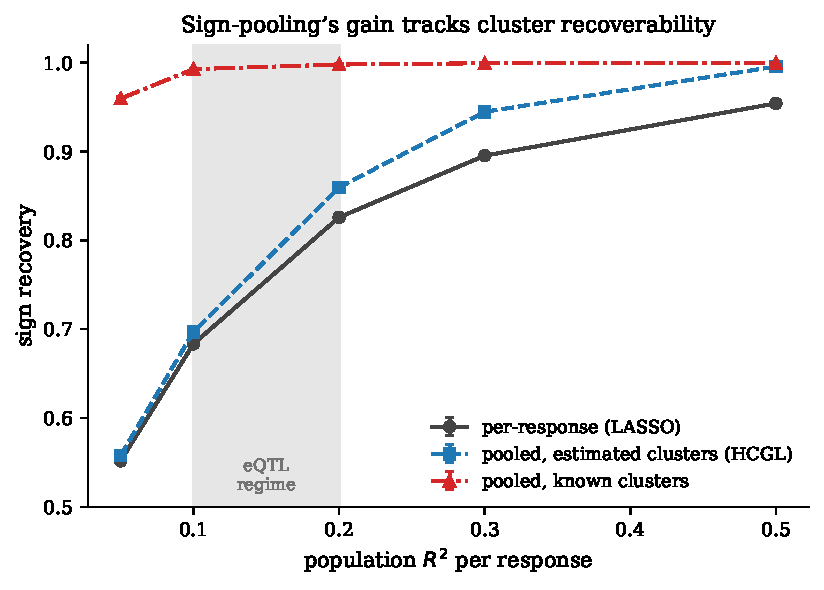
\includegraphics[width=0.72\linewidth]{figS1_recoverability.pdf}
	\caption{Sign-pooling's gain over per-response derivation tracks cluster
		recoverability. Sign recovery against population $R^2$ at fixed $T = 80$, for
		per-response derivation, estimated-cluster pooling (HCGL), and known-cluster
		pooling. The shaded band marks the $R^2$ range of the eQTL application of
		Section~\ref{sec:eqtl}. Points are means over $200$ replications, and error bars show
		one standard error.}
	\label{fig:recoverability}
\end{figure}

Pooling helps most when the sample is small relative to the structure.
Table~\ref{tab:regime} crosses the population $R^2$ with the sample size $T$.
The gap reaches $0.069$ at $R^2 = 0.30$ and $T = 60$ ($0.919$ against $0.850$).
The gap closes as $T$ grows, falling to $0.003$ at $T = 240$, because the
per-response derivation becomes consistent on its own once the sample is large.
The practical reading is that pooling earns its keep in the scarce-sample
regime, and adds little when the per-response signs already clear the gate.

\begin{table}[t]
	\centering
	\caption{Pooling's advantage is largest when structure is recoverable and the
		sample is small. Sign recovery for estimated-cluster pooling (HCGL) and
		per-response derivation across population $R^2$ and sample size $T$, with their
		difference (Gap). All other settings as in the base configuration. Cells are means over
		$200$ replications.}
	\label{tab:regime}
	\begin{tabular}{ccccc}
\toprule
$R^2$ & $T$ & Pooled (HCGL) & Per-response & Gap \\
\midrule
0.10 & 60 & 0.646 & 0.624 & +0.022 \\
0.10 & 120 & 0.765 & 0.764 & +0.001 \\
0.10 & 240 & 0.887 & 0.887 & +0.000 \\
\addlinespace
0.30 & 60 & 0.919 & 0.850 & +0.069 \\
0.30 & 120 & 0.969 & 0.945 & +0.024 \\
0.30 & 240 & 0.989 & 0.986 & +0.003 \\
\addlinespace
0.50 & 60 & 0.992 & 0.925 & +0.066 \\
0.50 & 120 & 0.999 & 0.980 & +0.019 \\
0.50 & 240 & 1.000 & 0.997 & +0.003 \\
\bottomrule
\end{tabular}
\end{table}

\subsection{The noise-floor gate} \label{sec:sim-gate}

The threshold $\tau$ trades recovered true signs for false-sign control along a
smooth frontier. Figure~\ref{fig:gate} plots sensitivity against the false-sign
rate as $\tau$ varies from $0.5$ to $3.5$, under known-cluster pooling. At
$\tau = 0.75$ the gate recovers $0.993$ of true signs but admits a false-sign
rate of $0.579$. At $\tau = 2.5$ it recovers $0.863$ of true signs at a
false-sign rate of $0.070$. The frontier bends near $\tau = 2.0$ to $2.5$, which
we read as the useful operating range for a final sign report. The package
default of $0.75$ is permissive by design, since it suits a screening step that
removes the worst noise-driven constraints before regularization.

\begin{figure}[t]
	\centering
	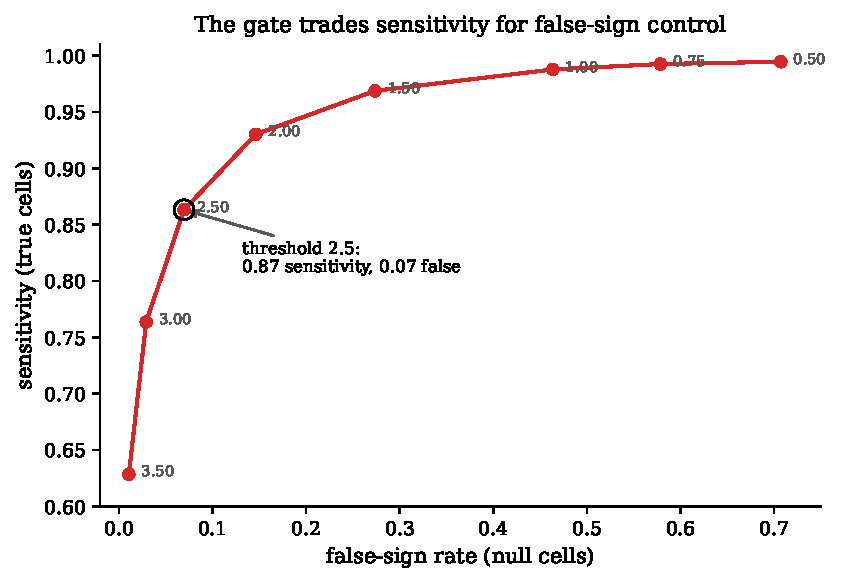
\includegraphics[width=0.72\linewidth]{figS2_gate_roc.pdf}
	\caption{The gate trades sensitivity for false-sign control along a smooth
		frontier. Sensitivity (recovery on true signals) against the false-sign rate
		(on null cells) as the threshold $\tau$ varies from $0.5$ to $3.5$, under
		known-cluster pooling in the base configuration. Labels give $\tau$, and the circled
		point ($\tau = 2.5$) marks the operating range. Means over $200$ replications.}
	\label{fig:gate}
\end{figure}

The over-dispersion is the design effect, which can be removed. The pooled
standard error divides by the cluster size as if the responses were independent,
which omits the factor $1 + (|\mathcal{C}|-1)\bar{\rho}$. A
design-effect-corrected gate scales the standard error by the square root of this
factor. The corrected gate brings the known-cluster false-sign rate from $0.579$
to $0.457$, matching the per-response $2\Phi(-\tau) = 0.453$, at a recovery cost
from $0.993$ to $0.988$ (replication code). At this matched false-sign rate near
$0.45$, known-cluster pooling recovers $0.988$ against $0.683$ for the per-response
derivation, so the recovery advantage does not come from the higher false-sign
rate. The correction leaves the flip rate
unchanged, because the marginal-versus-partial disagreement of
Section~\ref{sec:sim-correlated} is a bias rather than a variance. We keep the
uncorrected gate as the default screen before regularization, and recommend the
design-effect-corrected gate when the signs are reported as a final, calibrated
result.

The design effect also bounds the realized pooling gain. The base design draws
independent within-cluster residuals, for which $\bar{\rho} \approx 0$. We
correlate the residuals within each cluster and sweep $\bar{\rho}$, holding the
base configuration fixed (Table~\ref{tab:rhobar}). As $\bar{\rho}$ rises, the
known-cluster recovery falls from $0.990$ to $0.863$ and the false-sign rate
rises from $0.577$ to $0.809$. The design effect lowers the pooled effective
sample below $m\,T$, which drives both moves. The realized rate factor falls
from $\sqrt{m}$ toward one, so the gain is largest when the cluster carries
shared signal with weakly correlated residuals.

\begin{table}[t]
	\centering
	\caption{The pooling gain attenuates as within-cluster residual correlation
		rises. Known-cluster sign recovery, abstention, and false-sign rate against the
		within-cluster residual correlation $\bar{\rho}$, in the base configuration
		($N = 60$, $M = 20$, $G = 6$, $T = 80$, $R^2 = 0.10$, $\tau = 0.75$, cluster
		size $m = 10$). The rate factor $\sqrt{m / (1 + (m-1)\bar{\rho})}$ is the
		realized multiple of the per-response convergence rate against the ideal
		$\sqrt{m} = 3.16$. Means over $100$ replications.}
	\label{tab:rhobar}
	\begin{tabular}{ccccc}
\toprule
$\bar{\rho}$ & Recovery & Abstention & False-sign & Rate factor \\
\midrule
0.0 & 0.990 & 0.010 & 0.577 & 3.16 \\
0.3 & 0.939 & 0.050 & 0.718 & 1.64 \\
0.6 & 0.898 & 0.067 & 0.777 & 1.25 \\
0.9 & 0.863 & 0.082 & 0.809 & 1.05 \\
\bottomrule
\end{tabular}
\end{table}

The threshold also sets a multiplicity budget. The gate screens $N \times M$
cells. At threshold $\tau$ the gate admits a null cell with probability about
$2\Phi(-\tau)$. The expected number of false constraints is therefore about
$2\Phi(-\tau)\, N M$, which the default $\tau = 0.75$ leaves large and
$\tau = 2.5$ controls. A user with a target false-sign rate reads $\tau$ from the
frontier of Figure~\ref{fig:gate}. A user with a per-family budget sets
$2\Phi(-\tau) N M$ to the tolerated count.

The discovered clusters are stable across the cutoff fraction. Sign recovery for
estimated-cluster pooling runs from $0.683$ at $\rho_{\mathrm{cut}} = 0.3$ to
$0.724$ at $\rho_{\mathrm{cut}} = 0.7$, with no cliff. A low cutoff merges few
responses and reduces to the per-response derivation, while a high cutoff pools
more aggressively and trades false signs for recovery. The default
$\rho_{\mathrm{cut}} = 0.5$ sits at the midpoint of this range.

\subsection{Sign consistency} \label{sec:sim-consistency}

Pooling reaches sign consistency at a far smaller sample. Figure~\ref{fig:consistency}
shows sign recovery against the sample size $T$ at fixed $R^2 = 0.10$. Both
derivations are sign-consistent, since recovery rises toward one as $T$ grows.
Known-cluster pooling reaches $1.000$ by $T = 160$, while the per-response
derivation needs $T = 640$ to reach $0.979$. Pooling attains consistency at
roughly a quarter of the sample size. Appendix~\ref{app:theory} states the rate
that this curve illustrates.

\begin{figure}[t]
	\centering
	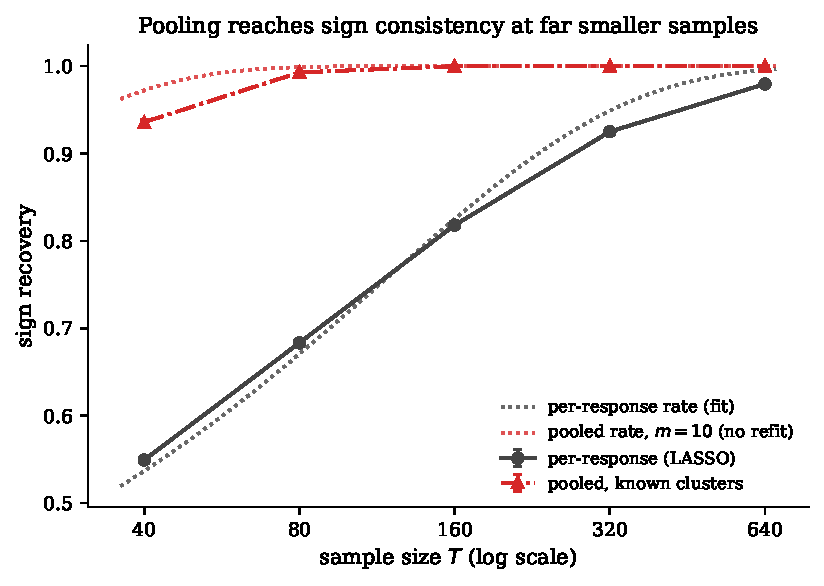
\includegraphics[width=0.72\linewidth]{figS4_consistency.pdf}
	\caption{Pooling reaches sign consistency at far smaller samples. Sign recovery
		against sample size $T$ (log scale) at fixed $R^2 = 0.10$, for per-response
		derivation and known-cluster pooling. Both rates approach one, and pooling
		reaches it sooner. Means over $200$ replications, and error bars show one standard
		error. The dotted curves are the Gaussian-gate rate $\Phi(c\sqrt{T} - \tau)$ implied
		by Appendix~\ref{app:theory}: the constant $c$ is fit to the per-response points, and
		the pooled curve applies the same $c$ at the cluster-size sample scaling $m\,T$
		($m = 10$) with no further fit. The ideal leads the data because the $m\,T$ scaling assumes a homogeneous
		within-cluster effect, while the simulated loadings are heterogeneous (magnitudes drawn from $U[0.5, 1.5]$),
		which lowers the pooled effective sample below $m\,T$ even at the near-zero residual correlation of the
		base design (Appendix~\ref{app:theory}).}
	\label{fig:consistency}
\end{figure}

The same contrast is visible cell by cell. Figure~\ref{fig:signmat} shows the
three sign matrices for one replication at $R^2 = 0.20$ and $\tau = 2.0$. The
known-cluster matrix reproduces the population signs as coherent within-cluster
blocks. The per-response matrix is fragmented, with isolated cells and
within-cluster sign alternations on the active predictors. Pooling removes the
alternations by sharing one decision across each cluster.

\begin{figure}[t]
	\centering
	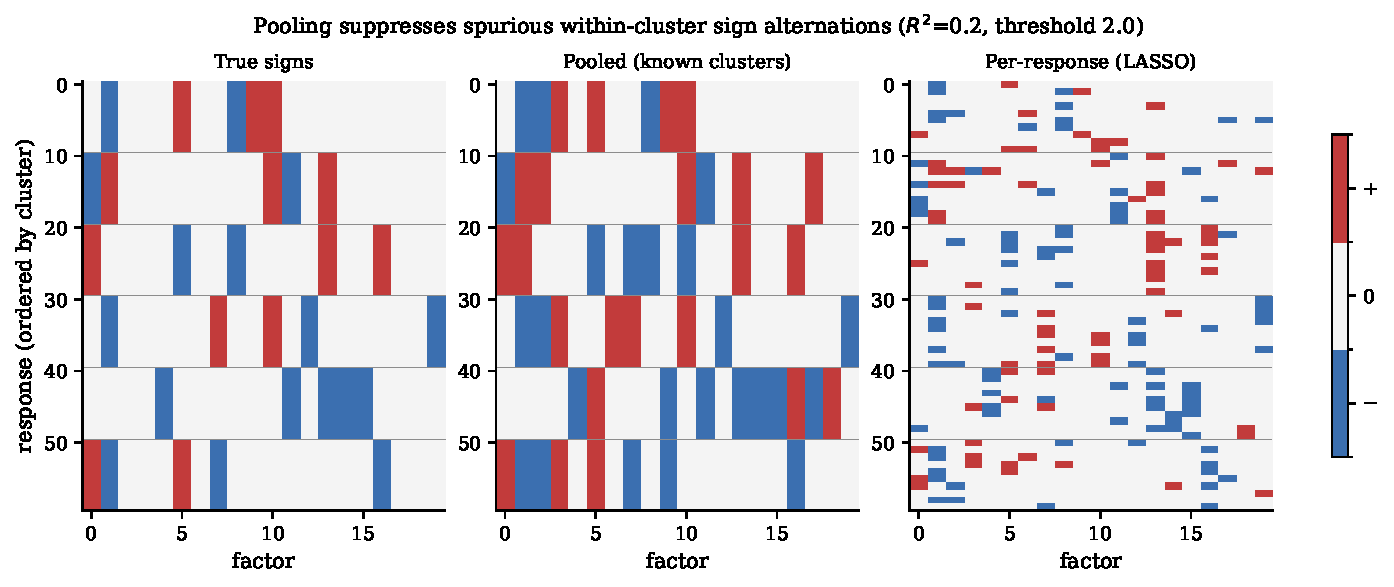
\includegraphics[width=\linewidth]{figS3_sign_matrices.pdf}
	\caption{Pooling suppresses spurious within-cluster sign alternations.
		Population signs (left), known-cluster-pooled signs (center), and per-response
		signs (right) for one replication at $R^2 = 0.20$ and $\tau = 2.0$. Rows are
		responses ordered by cluster, and columns are predictors. Blue, white, and red
		denote $-1$, $0$, and $+1$. Horizontal lines separate clusters.}
	\label{fig:signmat}
\end{figure}

\subsection{Correlated predictors and the marginal-sign assumption}
\label{sec:sim-correlated}

The method derives a sign from a marginal slope but imposes it on a partial
coefficient. Condition (A6) of Appendix~\ref{app:theory} asks the two to agree,
which holds when the predictors are uncorrelated. The base design draws
independent predictors, so (A6) holds by construction. We now correlate the
predictors to stress it.

We draw the factors with equicorrelation $\rho_X$ and sweep $\rho_X$ from $0$ to
$0.8$, holding the rest of the base configuration fixed.
Figure~\ref{fig:correlated} reports the three sign rates. As $\rho_X$ rises,
cross-predictor leakage pulls the marginal slope away from the partial
coefficient. The derived sign then flips. The sign-flip rate rises for every
derivation. Pooling amplifies it. At $\rho_X = 0.8$ the known-cluster flip rate
is $0.296$ against $0.217$ for the per-response derivation. The false-sign rate
saturates near one, because correlated predictors give null cells a spurious
marginal association.

A wrong marginal sign is more costly than an abstention. The constraint forces
the partial coefficient into the wrong half-space, an asymmetric and confident
error. Pooling sharpens the wrong sign as readily as the right one. The recovery
advantage of known-cluster pooling narrows sharply as $\rho_X$ rises, from $0.31$
at $\rho_X = 0$ to $0.05$ at $\rho_X = 0.8$. Above $\rho_X \approx 0.5$ the pooled
flip rate exceeds the per-response rate, so pooling trades a small recovery edge
for more confident errors. Cluster-pooled sign derivation suits weakly correlated
predictors. Under strong predictor correlation the marginal sign becomes
unreliable. A soft penalty that the data can overrule then recovers more signs,
at the cost of asserting more wrong ones.

We benchmark the hard sign constraint against the cooperative LASSO of
\citet{Chiquet+Grandvalet+Charbonnier:2012}, a soft penalty that couples the
signs of a cluster but lets the data overrule them. We fit both on the known
clusters across the same $\rho_X$ grid and select each penalty to minimize
coefficient error. We read the sign from the fitted coefficient
(Table~\ref{tab:coop}), not from the derived sign of
Figure~\ref{fig:correlated}. A wrong derived sign holds the coefficient in the
wrong half-space, where the penalty then drives it to zero. The fitted cell reads
as an abstention rather than a flip. The two methods make different kinds of error. The hard constraint never asserts
a wrong sign, holding its flip rate at $0.006$ or below across the grid. It
abstains instead, and its abstention reaches $0.887$ at $\rho_X = 0.8$ as the
marginal signal becomes unreliable. The cooperative LASSO commits to a sign on
almost every cell, so it asserts a wrong sign on $0.101$ to $0.220$ of cells as
leakage grows. It recovers more signs in exchange, from $0.895$ to $0.771$ across
the grid, against $0.743$ to $0.109$ for the hard constraint. It also reaches
lower coefficient error throughout. An abstention assigns no sign, but a
flip pins a coefficient to the wrong half-space. For a method whose output is a
sign, the two are not the same error.

\begin{table}[t]
	\centering
	\caption{The hard sign constraint never asserts a wrong sign, while the
		cooperative LASSO reaches higher recovery and lower coefficient error by flipping
		10\% to 22\% of signs. Sign recovery, flip rate,
		and abstention on active cells, with the coefficient mean squared error
		($\beta$-MSE), for a hard sign-constrained fit and the cooperative LASSO of
		\citet{Chiquet+Grandvalet+Charbonnier:2012}, both on known clusters, against the
		predictor equicorrelation $\rho_X$, in the base configuration. Each penalty
		minimizes $\beta$-MSE, and the sign is read from the fitted coefficient. Means
		over $40$ replications.}
	\label{tab:coop}
	\begin{tabular}{ccccccccc}
\toprule
 & \multicolumn{4}{c}{Hard sign constraint} & \multicolumn{4}{c}{Cooperative LASSO} \\
\cmidrule(lr){2-5} \cmidrule(lr){6-9}
$\rho_X$ & Rec. & Flip & Abst. & $\beta$-MSE & Rec. & Flip & Abst. & $\beta$-MSE \\
\midrule
0.0 & 0.743 & 0.000 & 0.257 & 0.0044 & 0.895 & 0.101 & 0.004 & 0.0026 \\
0.2 & 0.598 & 0.002 & 0.400 & 0.0046 & 0.895 & 0.099 & 0.005 & 0.0028 \\
0.4 & 0.487 & 0.005 & 0.508 & 0.0053 & 0.889 & 0.101 & 0.010 & 0.0032 \\
0.6 & 0.257 & 0.006 & 0.738 & 0.0071 & 0.857 & 0.131 & 0.012 & 0.0044 \\
0.8 & 0.109 & 0.004 & 0.887 & 0.0109 & 0.771 & 0.220 & 0.009 & 0.0084 \\
\bottomrule
\end{tabular}
\end{table}

The eQTL application of Section~\ref{sec:eqtl} sits below the adversarial regime.
The screened markers retain some linkage correlation. We collapse tight-linkage
runs to reduce it, so the design correlation is modest rather than extreme.

\begin{figure}[t]
	\centering
	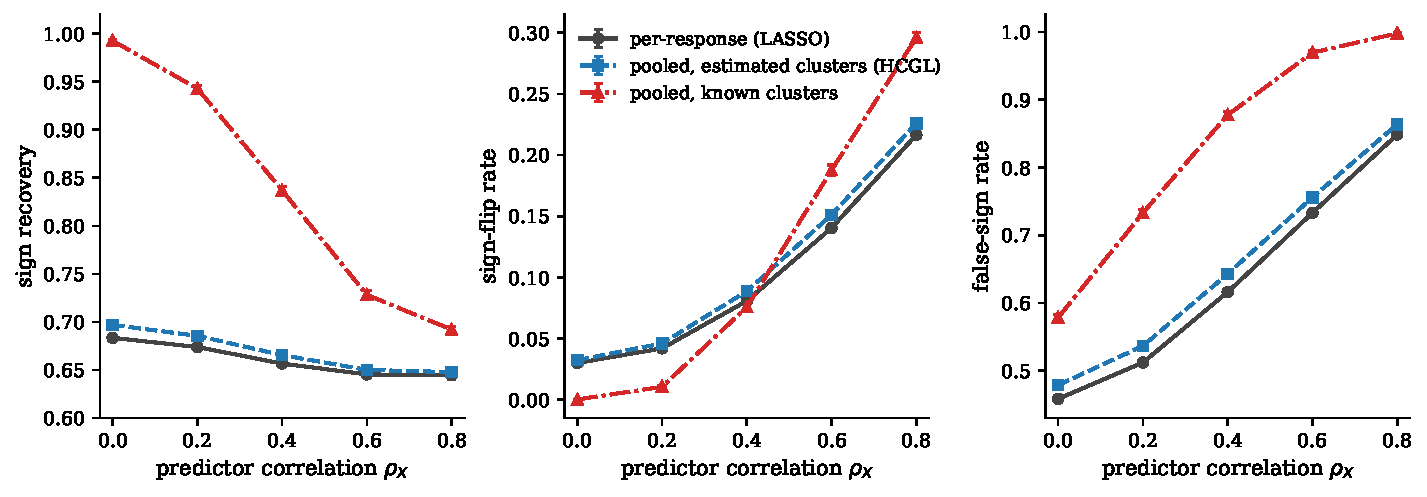
\includegraphics[width=\linewidth]{figS5_correlated.pdf}
	\caption{Cluster-pooled sign derivation degrades under correlated predictors.
		Sign recovery (left), sign-flip rate (center), and false-sign rate (right)
		against the predictor equicorrelation $\rho_X$, for per-response derivation,
		estimated-cluster pooling (HCGL), and known-cluster pooling, in the base
		configuration ($N = 60$, $M = 20$, $G = 6$, $T = 80$, $R^2 = 0.10$,
		$\tau = 0.75$). Predictors are drawn with equicorrelation $\rho_X$, which makes
		the marginal pooled slope disagree in sign with the partial coefficient. Means
		over $200$ replications, and error bars show one standard error.}
	\label{fig:correlated}
\end{figure}

These results locate the value of cluster-pooled sign derivation. Pooling helps
when the responses carry recoverable cluster structure and the sample is too
small for per-response signs to clear the gate. Pooling adds little when the sample is large or the clusters are invisible.
Pooling can hurt when the predictors are strongly correlated, because it sharpens
a flipped marginal sign into a wrong constraint. The threshold $\tau$, not the
pooling, governs the false-sign rate, so a user tunes the two concerns
separately. A user with a known grouping gains the most, and a user relying on
discovered clusters gains in proportion to how clearly the data reveal them.

\section{Application to yeast eQTL data} \label{sec:eqtl}

We apply the method to a yeast expression quantitative trait locus (eQTL) data
set, where the responses are gene expression levels and the predictors are
genetic markers. The application illustrates the method on real data. We examine whether real
responses carry the sign-coherent cluster structure that the method exploits. We
then read the recovered structure against known biology. We choose a data set that sits
in the low-recoverability regime of Section~\ref{sec:simulation}, so we report
interpretable structure rather than a prediction gain.

\subsection{Data and setup} \label{sec:eqtl-data}

The data come from a cross of two yeast strains \citep{Brem+Kruglyak:2005}, with
$T = 112$ segregants. We study the genes of the mitogen-activated protein kinase
(MAPK) signaling pathway, which divides into four sub-pathways, namely the
pheromone response, filamentation, high-osmolarity response, and cell-wall
integrity. We take the KEGG pathway membership measured in the data, which gives
$N = 64$ genes.\footnote{We use the KEGG MAPK membership measured in the data
	for reproducibility. The conditional-Gaussian-graphical-model literature
	\citep{Yin+Li:2011} works with a canonical $54$-gene MAPK subset. We keep the
	full measured membership here.} We reduce the marker panel from
$3244$ markers to representative markers by collapsing consecutive runs in tight
linkage, then keep the markers associated with at least two genes at
$p \le 0.01$, the screen of \citet{Yin+Li:2011}. The screen leaves $M = 202$
markers. We standardize the genes and the markers, and fit estimated-cluster
pooling at cutoff $\rho_{\mathrm{cut}} = 0.7$ and threshold $\tau = 2.0$, within the
operating range identified in Section~\ref{sec:sim-gate}.

\subsection{Recovered clusters and sign coherence} \label{sec:eqtl-clusters}

The discovered clusters are sign-coherent. The method recovers nine gene
clusters. Within each cluster, the genes agree on the marginal sign of their
marker associations. The agreement reaches $0.93$ of the cells that carry a
significant association at $p \le 0.05$ (Table~\ref{tab:clusters}). The agreement is a within-cluster consistency check, not independent validation.
The method forms the clusters from the same correlations that drive the shared
sign, then computes the agreement on the significant cells alone. The agreement
still shows that the discovered groups carry a single sign direction on these
data. The per-cluster agreement ranges from $0.84$
to $1.00$. The residual correlation within the clusters, after removing the marker
signal, averages $0.22$, against a total within-cluster correlation of $0.36$.
The residual correlation governs the realized pooling gain through the design
effect of Section~\ref{sec:sim-gate}, and it runs below the total correlation
that drives the clustering. At the typical cluster size, the clusters realize
about $1.7$ times the per-response convergence rate, below the ideal $\sqrt{m}$
of $2.7$.

The clusters track the sub-pathways only in part. The adjusted Rand index
between the clusters and the four sub-pathways is $0.114$, and the mean cluster
purity is $0.614$ (Table~\ref{tab:clusters}). The two pheromone-response
clusters are clean, at purity $1.00$ and $0.90$, while the cell-wall and
osmolarity genes mix across clusters. Co-expression groups the genes by shared
regulation, which need not follow the pathway annotation.
Figure~\ref{fig:clusters} orders the gene correlation matrix by cluster and
colors each gene by its sub-pathway.

\begin{table}[t]
	\centering
	\caption{Recovered gene clusters are sign-coherent within, and partly aligned to
		the MAPK sub-pathways. For each discovered cluster: the number of genes, the
		dominant sub-pathway with its purity, the number of markers with a nonzero
		loading on any cluster gene, and the within-cluster raw marginal-sign agreement.
		Yeast eQTL cross of \citet{Brem+Kruglyak:2005}: $64$ MAPK genes, $202$ markers,
		$112$ segregants. Estimated-cluster pooling at $\rho_{\mathrm{cut}} = 0.7$ and
		$\tau = 2.0$.}
	\label{tab:clusters}
	\begin{tabular}{cccccc}
\toprule
Cluster & Genes & Dominant sub-pathway & Purity & Markers & Sign coherence \\
\midrule
1 & 5 & Hog1 & 0.60 & 59 & 0.92 \\
2 & 8 & Hog1 & 0.50 & 57 & 0.84 \\
3 & 4 & Slt2 & 0.50 & 51 & 0.89 \\
4 & 7 & Kss1 & 0.43 & 62 & 0.97 \\
5 & 7 & Hog1 & 0.71 & 120 & 1.00 \\
6 & 6 & Slt2 & 0.50 & 86 & 0.95 \\
7 & 13 & Slt2 & 0.38 & 79 & 0.90 \\
8 & 4 & Fus3 & 1.00 & 41 & 1.00 \\
9 & 10 & Fus3 & 0.90 & 116 & 0.94 \\
\bottomrule
\end{tabular}
\end{table}

\begin{figure}[t]
	\centering
	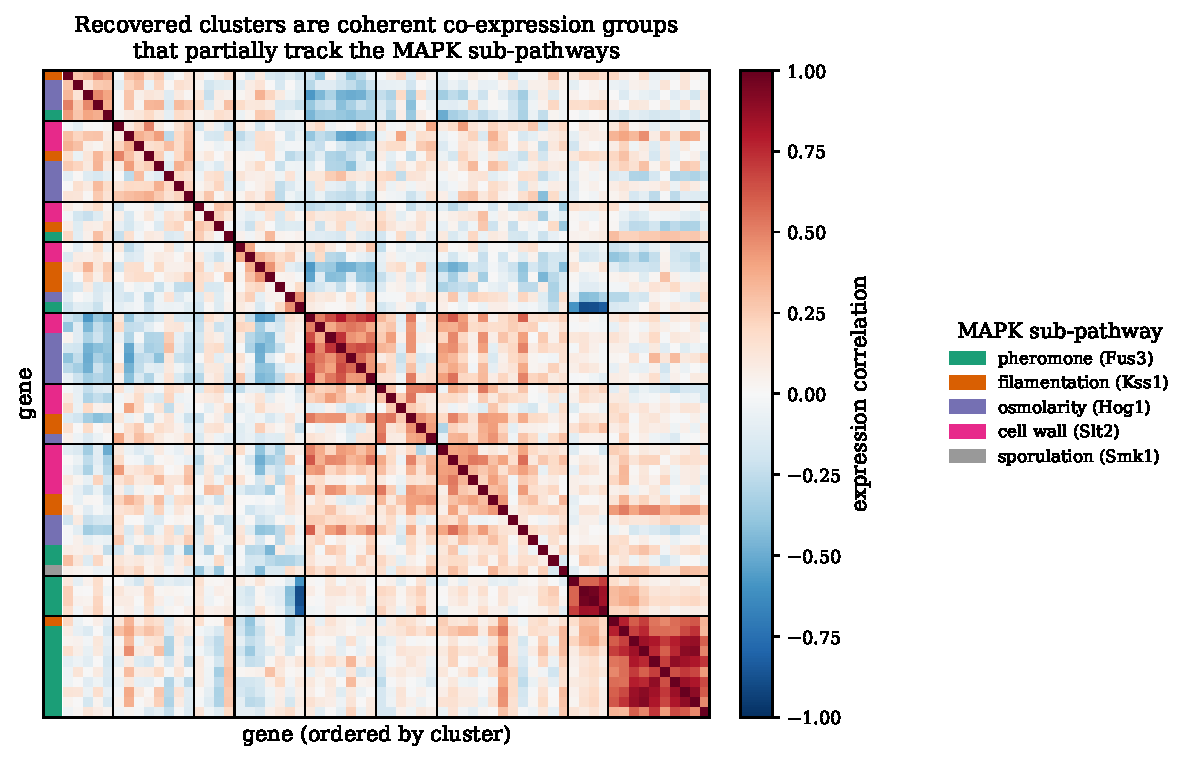
\includegraphics[width=0.78\linewidth]{figE1_clusters.pdf}
	\caption{Recovered clusters are coherent co-expression groups that partially
		track the MAPK sub-pathways. Expression correlation among the $64$ MAPK genes,
		ordered by discovered cluster, with the sub-pathway of each gene shown in the
		left bar. Black lines separate clusters. Yeast eQTL data of
		\citet{Brem+Kruglyak:2005}.}
	\label{fig:clusters}
\end{figure}

\subsection{Genomic structure} \label{sec:eqtl-genome}

The gated signs form coherent blocks along the genome.
Figure~\ref{fig:signs} shows the gated sign matrix, with genes ordered by
cluster and markers ordered along the genome. The signs form coherent
horizontal blocks within each cluster, the structure that the agreement
statistic measures. The gate leaves many cells at zero, where the pooled
evidence falls below $\tau$.

\begin{figure}[t]
	\centering
	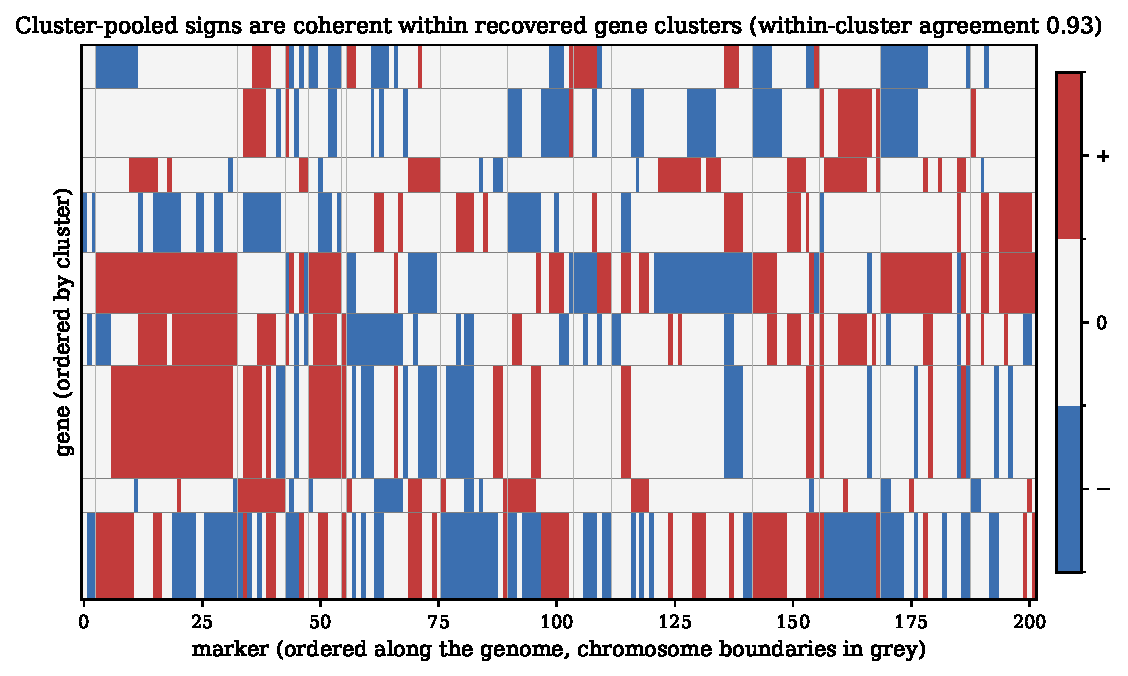
\includegraphics[width=\linewidth]{figE2_signs.pdf}
	\caption{Cluster-pooled signs are coherent within recovered gene clusters.
		Gated sign matrix for the $64$ genes (rows, ordered by cluster) against the
		$202$ markers (columns, ordered along the genome). Blue, white, and red denote
		$-1$, $0$, and $+1$, and grey lines mark chromosome boundaries. The
		within-cluster sign agreement is $0.93$.}
	\label{fig:signs}
\end{figure}

The marker loadings concentrate at a few genomic positions.
Figure~\ref{fig:hotspots} counts, for each marker, the genes that load on it. A
locus on chromosome $14$ loads $42$ of the $64$ genes, and loci on chromosomes
$12$, $3$, and $5$ each load more than $30$. The peaks recover the trans-acting
eQTL hotspots that regulate many genes at once, a documented feature of this
cross \citep{Brem+Kruglyak:2005}.

\begin{figure}[t]
	\centering
	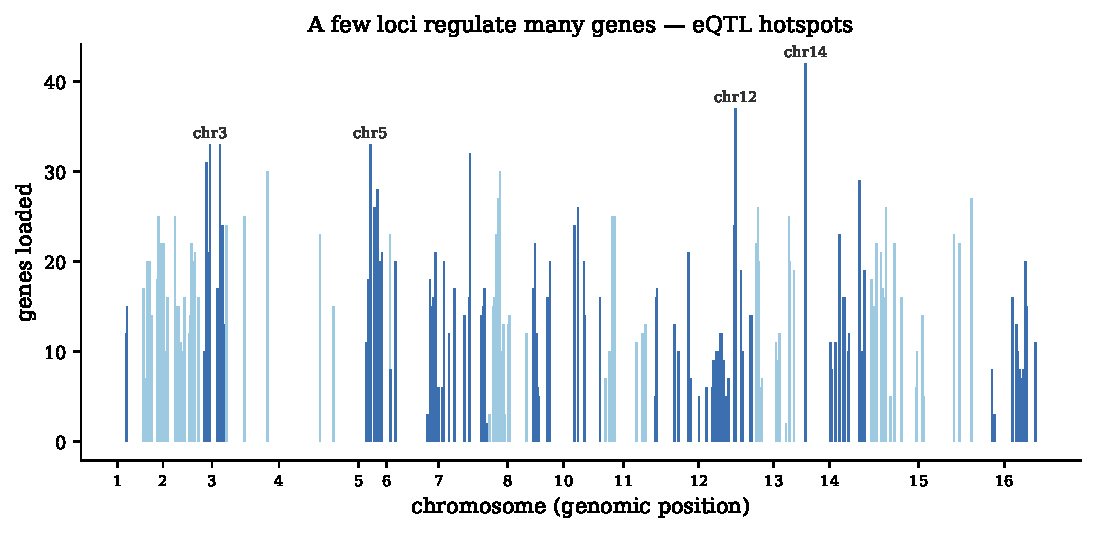
\includegraphics[width=\linewidth]{figE3_hotspots.pdf}
	\caption{A few loci regulate many genes, the eQTL hotspots. Number of genes
		loading on each marker against genomic position, for the $202$ screened markers.
		Alternating shades separate chromosomes, and the top four loci are labeled.
		Yeast eQTL data of \citet{Brem+Kruglyak:2005}.}
	\label{fig:hotspots}
\end{figure}

\subsection{Prediction} \label{sec:eqtl-prediction}

Pooling does not improve prediction on these data. In three-fold
cross-validation the per-response LASSO attains a median out-of-sample $R^2$ of
$0.118$ per gene, against $0.088$ for the factor-cluster variant and $0.038$ for
HCGL. The ranking matches the simulation. At the recoverability of this data
set, pooling sign constraints over weakly separated clusters constrains the fit
without a prediction payoff. The contribution here is the coherent, gated sign
structure rather than the forecast.

The discovered clusters are sign-coherent and map onto interpretable genomic
hotspots. The lower out-of-sample prediction marks the boundary of the method. A
user adopts cluster-pooled sign derivation for coherent, interpretable structure
in the small-sample regime, and not for a forecast gain where per-response signs
already suffice.
%% =====================================================================
\section{Discussion} \label{sec:discussion}

We develop a sign-derivation mechanism for multi-output sparse regression and
establish when it helps. The mechanism pools the univariate sign across a
data-driven cluster and gates it by a closed-form test. The pooling raises the
per-cell sample size by the cluster size. In the base simulation the pooling
recovers the population sign in 99.3\% of active cells against 68.3\% for the
per-response derivation. The gain comes almost entirely from clearing true
signals that the per-response gate abstains on, a 0.7\% abstention rate against
28.7\%.

The gain depends on the regime. The advantage over per-response derivation tracks
cluster recoverability, and is largest when the sample is small relative to the
structure, with a gap of 0.069 at population $R^2 = 0.30$ and $T = 60$. The gain
vanishes as the sample grows, because the per-response signs become consistent on
their own. The threshold governs the false-sign rate along a smooth frontier,
with a sensitivity of 0.86 at a false-sign rate of 0.07 at $\tau = 2.5$, so a
user separates the pooling decision from the false-sign tolerance. Pooling
reaches sign consistency at roughly a quarter of the sample the per-response
derivation needs.

On yeast eQTL data the recovered gene clusters agree on the marginal sign in 93\%
of significant cells, so the structure the method pools over is present in real
data. The cluster-marker loadings concentrate at a few genomic positions, the
known trans-acting hotspots of the cross. Pooling does not improve prediction
here, at a median out-of-sample $R^2$ of 0.038 against 0.118 for the per-response
LASSO, which the low recoverability of the data predicts. The contribution on
this data set is interpretable sign structure rather than forecast accuracy.

The mechanism changes how a practitioner derives sign constraints. A practitioner
with a known grouping gains the most. Factor models for portfolio optimization
are one such setting, where the factor grouping is given. In that setting, sign
recovery keeps the estimated factor model economically tractable, which the
strategic and tactical allocation built on it requires \citep{sepp2026rosaa}. A
practitioner relying on discovered
clusters gains in proportion to how clearly the data reveal them, and should
question the marginal sign agreement condition first when the predictors carry
strong cross-predictor correlation of opposing sign. For the literature, the
result extends univariate sign guidance from a single response to a data-driven
cluster, and pairs it with a gate that treats the sign as a screen rather than an
unconditional constraint.

Two limitations remain. The oracle distribution of the constrained estimator is
stated as Conjecture~1 and not proved. The marginal-sign-agreement condition
fails under correlated predictors, where Section~\ref{sec:sim-correlated} shows
the derived sign flips and pooling amplifies it. In that regime a cooperative
LASSO, which the data can overrule, recovers more of the signs at lower
coefficient error than the hard constraint. The cost is a higher flip rate
(Section~\ref{sec:sim-correlated}). We benchmark against the per-response
derivation, the cluster-size-one special case, and the cooperative LASSO of
\citet{Chiquet+Grandvalet+Charbonnier:2012}.

%% =====================================================================
\appendix

\section{The closed-form SSR identity} \label{app:ssr}

This appendix derives the residual sum-of-squares identity of
Equation~\eqref{eq:ssr} and gives the full $t$~statistic.

\paragraph{Derivation.}
For predictor $j$, the pooled no-intercept slope $\hat{\beta}_j$ of
Equation~\eqref{eq:slope-pooled} satisfies the first-order condition
$\bm{x}_j^\top \bm{y}_{\mathrm{sum}} = N\, \hat{\beta}_j\, (\bm{x}_j^\top \bm{x}_j)$.
The pooled residual sum of squares aggregates the squared residuals of the $N$
per-response fits at the common slope $\hat{\beta}_j$,
%
\begin{align}
	\mathrm{SSR}_j
	&= \sum_{k=1}^{N} \bigl\| \bm{y}_k - \hat{\beta}_j\, \bm{x}_j \bigr\|_2^2
	= \sum_{k=1}^{N} \Bigl( \|\bm{y}_k\|_2^2
	- 2\, \hat{\beta}_j\, \bm{x}_j^\top \bm{y}_k
	+ \hat{\beta}_j^{\,2}\, \bm{x}_j^\top \bm{x}_j \Bigr) \notag \\
	&= \|\bm{Y}\|_F^2
	- 2\, \hat{\beta}_j\, \bm{x}_j^\top \bm{y}_{\mathrm{sum}}
	+ N\, \hat{\beta}_j^{\,2}\, \bm{x}_j^\top \bm{x}_j , \label{eq:ssr-expand}
\end{align}
%
using $\sum_k \|\bm{y}_k\|_2^2 = \|\bm{Y}\|_F^2$ and
$\sum_k \bm{x}_j^\top \bm{y}_k = \bm{x}_j^\top \bm{y}_{\mathrm{sum}}$.
Substituting the first-order condition
$\bm{x}_j^\top \bm{y}_{\mathrm{sum}} = N\, \hat{\beta}_j (\bm{x}_j^\top \bm{x}_j)$
into the middle term collapses Equation~\eqref{eq:ssr-expand} to
Equation~\eqref{eq:ssr},
$\mathrm{SSR}_j = \|\bm{Y}\|_F^2 - N\, \hat{\beta}_j^{\,2} (\bm{x}_j^\top \bm{x}_j)$.
The right-hand side requires only $\|\bm{Y}\|_F^2$ (computed once), the
per-predictor inner product $\bm{x}_j^\top \bm{x}_j$, and the slope, so the full
$(N, M)$ statistic is one matrix product rather than a loop that forms the
$T \times N$ residual matrix for each predictor.

\paragraph{Variance, standard error, and $t$~statistic.}
The pooled variance estimator, standard error, and $t$~statistic are
%
\begin{equation} \label{eq:tstat}
	\hat{\sigma}_j^{\,2} = \frac{\mathrm{SSR}_j}{N\, T - N},
	\qquad
	\widehat{\mathrm{SE}}\bigl(\hat{\beta}_j\bigr) =
	\sqrt{\frac{\hat{\sigma}_j^{\,2}}{N\, \bm{x}_j^\top \bm{x}_j}},
	\qquad
	t_j = \frac{\hat{\beta}_j}{\widehat{\mathrm{SE}}\bigl(\hat{\beta}_j\bigr)}.
\end{equation}
%
The cluster-pooled variant $t_{j, \mathcal{C}}$ used in the gate of
Equation~\eqref{eq:gate} substitutes $|\mathcal{C}|$ for $N$ throughout
Equation~\eqref{eq:tstat} and restricts the Frobenius norm to the cluster
columns, $\sum_{k \in \mathcal{C}} \|\bm{y}_k\|_2^2$. Missing entries are handled
by per-cell validity-mask accounting, which reduces to
Equation~\eqref{eq:tstat} when the data are fully observed
\citep{factorlasso-jss}.


\section{Conditions and proof for the sign-consistency result} \label{app:theory}

This appendix states the support-sign consistency of the cluster-pooled
sign-derivation mechanism and gives a proof sketch. The sign matrix is derived
identically under the HCGL and FCGL modes, which gate the same cluster-pooled
slope at the same threshold and differ only in the group norm of the penalty, so
the argument applies to both. We establish the support-sign statement
(Proposition~1) under conditions (A1)--(A6). The oracle distributional statement
that would accompany a full theorem, namely asymptotic normality on the true
support with OLS-equivalent covariance, is recorded as Conjecture~1 and not
proved here. The argument holds under stylized conditions rather than as a
guarantee for every regime. Condition (A6) below requires the marginal
cluster-pooled slope to agree in sign with the partial true coefficient, and
strong cross-predictor collinearity of opposing sign is exactly what breaks it.
Under such collinearity the asymptotic argument is not claimed to hold, and the
evidence for the mechanism in that regime is the simulation of
Section~\ref{sec:simulation}, not Proposition~1.

We adopt the notation of Section~\ref{sec:methods}. Let
$\bm{\beta}_{\mathrm{true}} \in \mathbb{R}^{N \times M}$ denote the true
coefficient matrix in the data-generating model
$\bm{Y} = \bm{X}\, \bm{\beta}_{\mathrm{true}}^\top + \bm{\varepsilon}$, and let
$\bm{S}_{\mathrm{true}} \in \{-1, 0, +1\}^{N \times M}$ be the matrix of true
signs, with $S_{\mathrm{true}, kj} = 0$ where $\beta_{\mathrm{true}, kj} = 0$.
Let $\hat{\bm{S}}_T$ denote the gated cluster-pooled sign matrix of
Equations~\eqref{eq:slope-cluster}--\eqref{eq:gate} at sample size $T$, and let
$\hat{\bm{\beta}}_T$ denote the constrained adaptive estimator of
Equation~\eqref{eq:sgl-sign} under $\hat{\bm{S}}_T$ with the adaptive weights of
Equation~\eqref{eq:adapt-cell}.

\paragraph{Regularity conditions.}
\begin{description}
	\item[(A1) Sub-Gaussian noise.] The residual matrix $\bm{\varepsilon}$ has
	independent rows with mean zero and finite variance, and each entry
	$\varepsilon_{tk}$ is sub-Gaussian with proxy variance bounded above by a fixed
	constant $\sigma^2_{\max}$.
	\item[(A2) Design regularity.] The predictor matrix $\bm{X}$ satisfies the moment
	condition $T^{-1}\, \bm{X}^\top \bm{X} \to \bm{\Sigma}_F$ as $T \to \infty$ with
	$\bm{\Sigma}_F$ positive definite, and the columns of $\bm{X}$ are bounded in
	probability.
	\item[(A3) Cluster sign coherence.] The HCGL partition recovered from
	$\operatorname{corr}(\bm{Y})$ respects the true within-cluster sign structure in
	the following sense. For every cluster $\hat{\mathcal{C}}$ discovered on the
	sample $(\bm{X}, \bm{Y})$ and every predictor $j$, the signs
	$\{S_{\mathrm{true}, kj} : k \in \hat{\mathcal{C}}, S_{\mathrm{true}, kj} \neq 0\}$
	share a single value. The condition is weaker than perfect cluster recovery,
	because the discovered partition need not match the true cluster identity, only
	respect the true sign structure.
	\item[(A4) Separation.] There exists a positive constant $c^\star$ such that, for
	every cluster $\mathcal{C}$ and every predictor $j$ with
	$\beta_{\mathrm{true}, kj} \neq 0$ for some $k \in \mathcal{C}$, the
	cluster-pooled population slope $\beta_{j, \mathcal{C}}^{\mathrm{pop}}$ satisfies
	$|\beta_{j, \mathcal{C}}^{\mathrm{pop}}| / \operatorname{SE}_T(\beta_{j, \mathcal{C}}^{\mathrm{pop}}) \to \infty$
	at rate at least $\sqrt{T}$, with margin
	$|\beta_{j, \mathcal{C}}^{\mathrm{pop}}| / \operatorname{SE}_T \geq \tau + c^\star$
	for all sufficiently large $T$.
	\item[(A5) Penalty rate.] The regularization strength satisfies $\lambda_T \to 0$
	and $\sqrt{T}\, \lambda_T \to \infty$ as $T \to \infty$. The adaptive exponent is
	$\gamma > 0$.
	\item[(A6) Marginal sign agreement on the support.] For every discovered cluster
	$\hat{\mathcal{C}}$ and every predictor $j$ with $S_{\mathrm{true}, kj} \neq 0$
	for some $k \in \hat{\mathcal{C}}$, the population cluster-pooled slope satisfies
	$\operatorname{sign}(\beta_{j, \hat{\mathcal{C}}}^{\mathrm{pop}}) = S_{\mathrm{true}, kj}$
	for every such $k$. The condition is substantive because the pooled slope is a
	\emph{marginal} quantity. With correlated predictors,
	$\beta_{j, \mathcal{C}}^{\mathrm{pop}} \propto
	\sum_{l} (\sum_{k \in \mathcal{C}} \beta_{\mathrm{true}, kl})\, \bm{\Sigma}_{F, jl}$,
	so cross-predictor leakage can flip the marginal sign away from the \emph{partial}
	sign that $\bm{S}_{\mathrm{true}}$ encodes. (A6) holds when the predictors are
	uncorrelated, and more generally when the cross-predictor leakage term does not
	dominate the own-predictor term. The mixed-sign regimes of
	Section~\ref{sec:simulation} probe the violations of (A3) and (A6).
\end{description}

\paragraph{Statement.}
Define the support-sign event
%
\begin{equation} \label{eq:thm-sign}
	\mathcal{H}_T \;=\;
	\Bigl\{\, \hat{S}_{T, kj} = S_{\mathrm{true}, kj}
	\;\;\text{for all $(k, j)$ with}\;\; S_{\mathrm{true}, kj} \neq 0 \,\Bigr\},
\end{equation}
%
the event that the gate neither pins a true-support cell to zero nor assigns it
the wrong half-space.
\begin{description}
	\item[Proposition 1 (support-sign and support consistency).] Under conditions
	(A1)--(A6), $\Pr(\mathcal{H}_T) \to 1$ as $T \to \infty$, and, conditional on
	this event, the constrained adaptive sparse group LASSO estimator
	$\hat{\bm{\beta}}_T$ recovers the true support,
	$\Pr\!\bigl(\operatorname{supp}(\hat{\bm{\beta}}_T) = \operatorname{supp}(\bm{\beta}_{\mathrm{true}})\bigr) \to 1$.
	\item[Remark (truly-zero cells and the fixed threshold).] Proposition~1 does not
	claim $\Pr(\hat{\bm{S}}_T = \bm{S}_{\mathrm{true}}) \to 1$. At a fixed threshold
	$\tau$, the stronger claim is false. On a cell where the population pooled slope
	is exactly zero, the per-response gate $t$~statistic is asymptotically standard
	normal, so the per-response gate retains the cell with limiting probability
	$2\Phi(-\tau) \approx 0.45$ at the default $\tau = 0.75$. The cluster-pooled gate
	retains such a cell with higher probability when the cluster's responses are
	correlated, because the pooled variance estimate of Equation~\eqref{eq:tstat}
	sums the $|\mathcal{C}|$ per-response residuals and does not adjust for the
	positive within-cluster correlation that pooling exploits, which over-disperses
	the pooled null $t$~statistic. The higher pooled false-sign rate in
	Section~\ref{sec:simulation} is this effect. On a cell where the partial coefficient is zero but the
	marginal pooled slope is not, through cross-predictor leakage, the gate retains
	the cell with probability tending to one. Both outcomes leave support recovery to
	the penalty. The retained constraint is a one-sided half-space whose boundary
	contains zero, so it never excludes the value $\hat{\beta}_{kj} = 0$ that the
	adaptive penalty drives the cell toward. A binding half-space on a truly-zero
	cell clips the unconstrained estimate's sampling noise on one side, a bounded
	bias of order the cell's standard error rather than a sign error. Exact recovery
	of $\bm{S}_{\mathrm{true}}$ would additionally require a diverging threshold,
	$\tau_T \to \infty$ with $\tau_T = o(\sqrt{T})$, together with zero marginal
	leakage on the off-support cells. We keep the fixed finite-sample default and
	treat the gate as a screen rather than a model-selection oracle.
	\item[Conjecture 1 (oracle distribution).] Under the same conditions, the
	restriction of $\sqrt{T}\, (\hat{\bm{\beta}}_T - \bm{\beta}_{\mathrm{true}})$ to
	the true support $\operatorname{supp}(\bm{\beta}_{\mathrm{true}})$ converges in
	distribution to a centered Gaussian with the same asymptotic covariance as the
	OLS estimator restricted to the true support. Establishing this requires
	verifying that the row-aggregated adaptive weights of the companion paper
	\citep{factorlasso-jss} inherit the divergence-on-zeros and
	boundedness-on-support rates of the \citet{Wang+Leng:2008} argument in the
	multi-response, sign-constrained setting. We do not prove it here.
\end{description}

\paragraph{Pooling rate.} The separation in (A4) is stated at the minimal
$\sqrt{T}$ rate, but pooling sharpens it. The gate statistic uses the closed-form
standard error of Equation~\eqref{eq:tstat}, which divides by
$\sqrt{|\mathcal{C}|\, \bm{x}_j^\top \bm{x}_j}$ and so pools the $|\mathcal{C}|$
cluster responses with the $T$ observations. For a cluster of size $m$ with
independent within-cluster residuals the effective sample size is $mT$, so the
support statistic diverges at the $\sqrt{mT}$ rate, a factor $\sqrt{m}$ above the
per-response $\sqrt{T}$ rate. Within-cluster residual correlation lowers the gain.
For a common residual correlation $\bar{\rho}$ the design effect
$1 + (m-1)\bar{\rho}$, the same factor that governs a clustered-sample mean,
reduces the effective sample to $mT / (1 + (m-1)\bar{\rho})$ and the realized rate
to $\sqrt{m / (1 + (m-1)\bar{\rho})}$. The realized rate equals $\sqrt{m}$ as
$\bar{\rho} \to 0$ and tends to one as $\bar{\rho} \to 1$, so the gain is largest
as $\bar{\rho} \to 0$. This residual correlation is distinct from the total
correlation that the clustering reads, so a coherent cluster need not carry a
large $\bar{\rho}$. Equation~\eqref{eq:tstat} estimates the variance as if
$\bar{\rho} = 0$, which both overstates the rate above and over-disperses the null
statistic, the source of the elevated false-sign rate of
Section~\ref{sec:simulation}. The divergence and hence Proposition~1 hold for any
$\bar{\rho} < 1$. Figure~\ref{fig:consistency} plots the $\sqrt{mT}$ ideal, which
the realized recovery approaches from below.

\paragraph{Proof sketch.}
The argument proceeds in four steps that mirror the layered mechanism.
Steps~1--3 establish $\Pr(\mathcal{H}_T) \to 1$. Step~4 sketches the conditional
support recovery and isolates what remains open for Conjecture~1.

\emph{Step 1 (slope consistency).} Under conditions (A1)--(A2), the
cluster-pooled univariate slope $\hat{\beta}_{j, \mathcal{C}}$ of
Equation~\eqref{eq:slope-cluster} satisfies
$\hat{\beta}_{j, \mathcal{C}} \to \beta_{j, \mathcal{C}}^{\mathrm{pop}}$ in
probability as $T \to \infty$ for every cluster $\mathcal{C}$ and predictor $j$.
The convergence applies the law of large numbers to the no-intercept OLS
estimator, using the sub-Gaussian tail bound on $\bm{\varepsilon}$ to control the
deviation rate.

\emph{Step 2 (no gating on the support).} The closed-form SSR identity of
Equation~\eqref{eq:ssr} produces a consistent variance estimator
$\hat{\sigma}_j^2 \to \sigma_{j, \mathrm{pop}}^2$ in probability. For every
$(j, \mathcal{C})$ pair on the support, the separation condition (A4) gives
$|t_{j, \mathcal{C}}| \to \infty$ in probability at rate $\sqrt{T}$, so
$\Pr(|t_{j, \mathcal{C}}| \geq \tau) \to 1$ and the probability that the gate
pins any true-support cell to zero vanishes. The step makes no claim about
off-support cells. At a fixed $\tau$ the gate retains an off-support cell with
non-vanishing probability, as the Remark notes, and the argument does not need it
to abstain.

\emph{Step 3 (correct signs on the support).} Steps 1 and 2 imply that for every
cluster $\hat{\mathcal{C}}$ discovered by HCGL and every support predictor $j$,
the derived sign $\operatorname{sign}(\hat{\beta}_{j, \hat{\mathcal{C}}})$
converges in probability to
$\operatorname{sign}(\beta_{j, \hat{\mathcal{C}}}^{\mathrm{pop}})$. The marginal
sign agreement condition (A6) equates this population sign with the common true
entry $S_{\mathrm{true}, kj}$, which is single-valued within the cluster by the
coherence condition (A3). The broadcasted sign therefore matches
$S_{\mathrm{true}, kj}$ for every $k \in \hat{\mathcal{C}}$ on the support, and
$\Pr(\mathcal{H}_T) \to 1$ follows from a union bound over the finitely many
$(j, \mathcal{C})$ pairs.

\emph{Step 4 (constrained adaptive support recovery).} Condition on the event
$\mathcal{H}_T$, which has probability tending to one by Step~3. On this event,
every true-support cell carries its correct half-space constraint, and the
support-restricted estimator is consistent by standard arguments, so the
constraint is inactive in the limit and the estimator coincides with the
unconstrained adaptive group LASSO on the support. Off-support cells carry either
a zero-pin, which enforces the truth directly, or a one-sided half-space
containing zero, which cannot exclude the target value and can bind only by
pushing the estimate toward zero. Under condition (A5), the adaptive reweighting
of Equation~\eqref{eq:adapt-cell} with $\gamma > 0$ produces weights that diverge
on truly-zero cells and remain bounded on truly-nonzero cells, which yields
support recovery by the standard adaptive-penalty argument. This establishes the
support-recovery claim of Proposition~1. The distributional claim of Conjecture~1
would require verifying that the row-aggregated adaptive weights of the companion
paper \citep{factorlasso-jss}, an RMS aggregation across the non-pinned
predictors of a response rather than a single per-coefficient weight as in the
original \citet{Wang+Leng:2008} setup, inherit the rate conditions their
central-limit argument needs in the multi-response, sign-constrained problem. We
leave this to future work.

\paragraph{Remarks.}
The cluster sign coherence condition (A3) and the marginal sign agreement
condition (A6) are the substantive sufficient conditions for the proof. (A3) is
weaker than the perfect-cluster-recovery condition that would require
$\hat{\mathcal{C}}_g = \mathcal{C}_g^\star$ for every cluster. It permits HCGL to
discover a partition that differs from the true clusters at the identity level,
as long as the discovered clusters respect the within-cluster sign structure.
(A6) is the price of deriving signs from marginal rather than partial evidence,
and it is the condition a practitioner should question first when the predictors
carry strong cross-predictor correlation of opposing sign. The application of
Section~\ref{sec:eqtl} shows that HCGL satisfies the coherence condition reliably
even when the adjusted Rand index against a reference grouping is moderate.
%% =====================================================================
\section{Computation and reproducibility} \label{app:computation}

The method is implemented in the open-source Python package \texttt{factorlasso}
\citep{factorlasso}, which expresses the sign-constrained sparse group LASSO of
Equation~\eqref{eq:sgl-sign} as a convex cone program. The simulation study of
Section~\ref{sec:simulation} is reproduced by the scripts
\texttt{sign\_pooling\_simulation.py} and \texttt{exhibits.py}, which regenerate
Tables~\ref{tab:base}--\ref{tab:coop} and
Figures~\ref{fig:recoverability}--\ref{fig:correlated} from a fixed random seed.
The eQTL application of Section~\ref{sec:eqtl} is reproduced by
\texttt{eqtl\_pipeline.py} and \texttt{eqtl\_exhibits.py}, which regenerate
Table~\ref{tab:clusters} and Figures~\ref{fig:clusters}--\ref{fig:hotspots}. The
yeast eQTL data are public \citep{Brem+Kruglyak:2005} and are distributed with
the \texttt{trigger} Bioconductor package. The reproduction bundle is openly
archived with a permanent identifier at
\url{https://doi.org/10.5281/zenodo.21000294}, and developed at
\url{https://github.com/ArturSepp/factorlasso/tree/main/papers/sign_pooling_2026}.
A pinned \texttt{requirements.txt} fixes every dependency,
including \texttt{factorlasso} version 0.7.2, so the reported
tables and figures regenerate from the fixed seed under the recorded environment.

%% =====================================================================
%% Back matter -- these sit BEFORE the reference list (CSDA guide, Article structure).
\section*{Declaration of competing interest}
Both authors are employed by LGT Bank. The bank had no role in the design of the
method, the analysis, or the decision to submit the work for publication. The
authors declare no other competing interest.

\section*{Funding}
This research did not receive any specific grant from funding agencies in the
public, commercial, or not-for-profit sectors.

\section*{Data availability}
The yeast eQTL data are publicly available \citep{Brem+Kruglyak:2005}. The
simulated data and the code that regenerates every table and figure are openly
available in the reproduction bundle at
\url{https://doi.org/10.5281/zenodo.21000294}, described in
Appendix~\ref{app:computation}.

%% AI-use disclosure -- Elsevier requires this given AI-assisted drafting.
\section*{Declaration of generative AI and AI-assisted technologies in the manuscript preparation process}
During the preparation of this work the authors used Anthropic's Claude Opus 4.8.
The model was used to assist with the design and development of the analysis
code (including the design of the implementation, drafting code, and reviewing and
debugging it) and, additionally, to draft and edit prose. After using this tool the
authors reviewed and edited all content and code as needed and take full
responsibility for the content of the publication.


\section*{Acknowledgements}
The authors thank colleagues at LGT Bank for feedback on the methodology
and its application to portfolio optimization and multi-asset capital market assumption estimation.

%% =====================================================================
\bibliographystyle{cas-model2-names}
\bibliography{refs}

\end{document}